\section{LSF}
\begin{figure}
	\centering
	\begin{minipage}{0.49\textwidth}
		\includegraphics[page=6,height=.3\textheight]{../data/analysis/lsf/gendet_ap1.pdf} 
		\includegraphics[page=6,height=.3\textheight]{../data/analysis/lsf/detspot_ap1.pdf} 
		\includegraphics[page=6,height=.3\textheight]{../data/analysis/lsf/detnbaut_ap1.pdf} 
		\caption{Relative state reduction of different automata using LSF.}
		\label{exp:fig:lsf_size_hist}
	\end{minipage}
	\hfill
	\begin{minipage}{0.49\textwidth}
		\includegraphics[page=2,height=.3\textheight]{../data/analysis/lsf/gendet_ap1.pdf} 
		\includegraphics[page=2,height=.3\textheight]{../data/analysis/lsf/detspot_ap1.pdf} 
		\includegraphics[page=2,height=.3\textheight]{../data/analysis/lsf/detnbaut_ap1.pdf} 
		\caption{Relative state reduction of different automata using LSF.}
		\label{exp:fig:lsf_reduct_abs}
	\end{minipage}
\end{figure}


\begin{figure}
	\centering
	\begin{minipage}{0.49\textwidth}
		\includegraphics[page=4,height=.3\textheight]{../data/analysis/lsf/gendet_ap1.pdf} 
		\includegraphics[page=4,height=.3\textheight]{../data/analysis/lsf/detspot_ap1.pdf} 
		\includegraphics[page=4,height=.3\textheight]{../data/analysis/lsf/detnbaut_ap1.pdf} 
		\caption{Relative state reduction of different automata using LSF.}
		\label{exp:fig:lsf_reduct_sccs}
	\end{minipage}
	\hfill
	\begin{minipage}{0.49\textwidth}
		\includegraphics[page=5,height=.3\textheight]{../data/analysis/lsf/gendet_ap1.pdf} 
		\includegraphics[page=5,height=.3\textheight]{../data/analysis/lsf/detspot_ap1.pdf} 
		\includegraphics[page=5,height=.3\textheight]{../data/analysis/lsf/detnbaut_ap1.pdf} 
		\caption{Relative state reduction of different automata using LSF.}
		\label{exp:fig:lsf_reduct_prios}
	\end{minipage}
\end{figure}

\begin{figure}
	\centering
	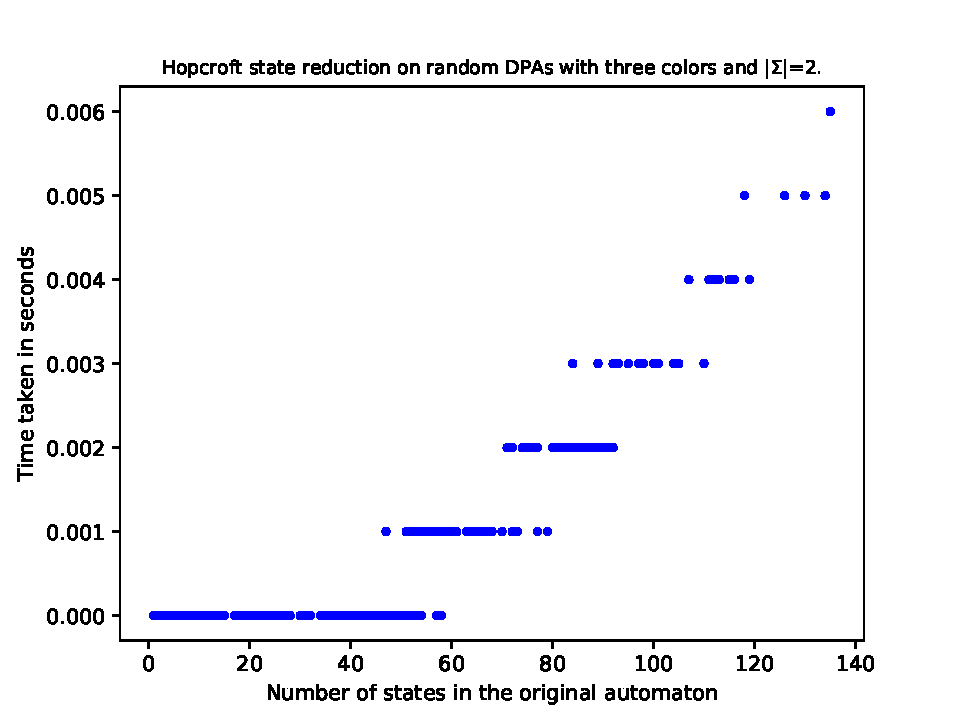
\includegraphics[page=1,height=.3\textheight]{../data/analysis/lsf/gendet_ap1.pdf} 
	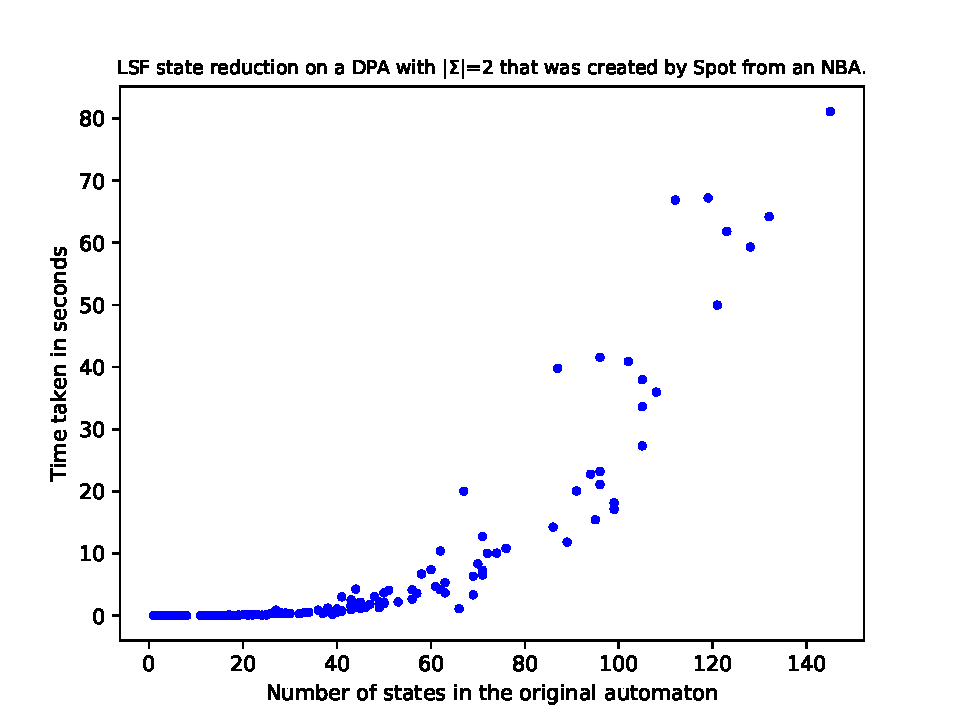
\includegraphics[page=1,height=.3\textheight]{../data/analysis/lsf/detspot_ap1.pdf} 
	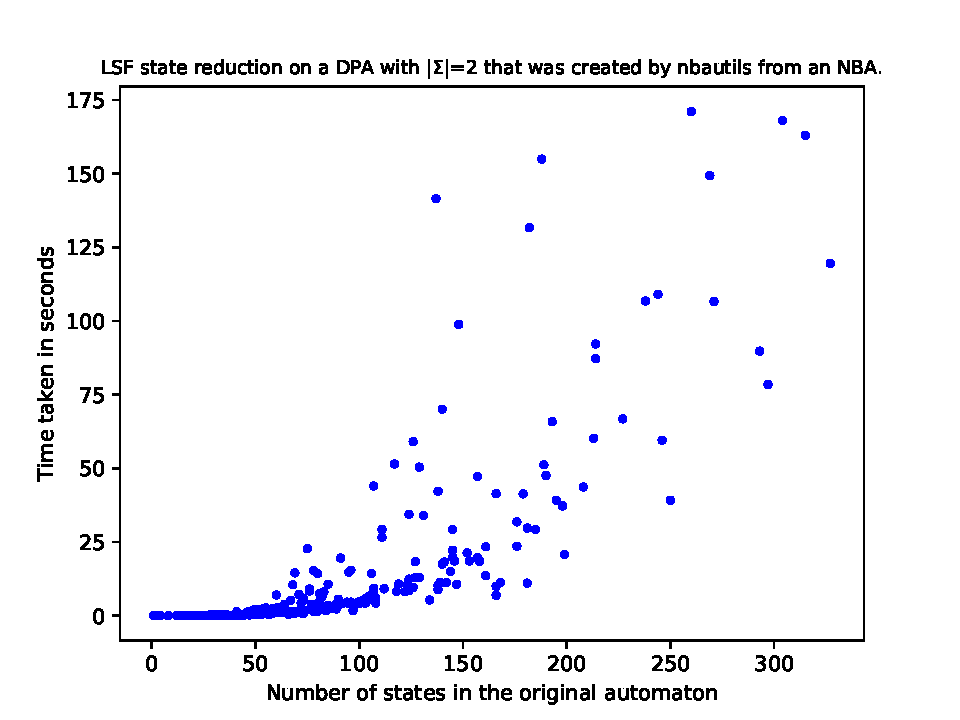
\includegraphics[page=1,height=.3\textheight]{../data/analysis/lsf/detnbaut_ap1.pdf} 
	\caption{Run time of LSF.}
	\label{exp:fig:lsf_time}
\end{figure}